% Slides of the threshold leanXMSS proof of concept. Build by `latexmk`.

\documentclass[t]{beamer}
\geometry{papersize={720bp,405bp}}
\usefonttheme{serif}\usefonttheme{professionalfonts}
\usepackage[no-math]{fontspec}
\usepackage{amsmath,outlines,tikz}

% Settings. Sizes: 12 bp text on a 22 bp line, 24 bp titles, the same at every list level.
\renewcommand{\normalsize}{\fontsize{12bp}{22bp}\selectfont}
\setbeamerfont{frametitle}{size=\fontsize{24bp}{30bp}\selectfont}
\setbeamerfont{itemize/enumerate subbody}{size=\normalsize}
\setbeamerfont{itemize/enumerate subsubbody}{size=\normalsize}
\setbeamercolor{structure}{fg=black}
\setbeamertemplate{navigation symbols}{}\setbeamertemplate{footline}{\vspace{7bp}}
\setbeamertemplate{frametitle}{\vspace{18bp}\strut\insertframetitle\vspace{-16bp}}
\setbeamertemplate{title page}{\vspace{125bp}\centering\usebeamerfont{frametitle}\inserttitle\par}
\setbeamertemplate{itemize items}{\strut--}
\setbeamerfont{footnote}{size=\fontsize{8bp}{14.4bp}\selectfont}
\setbeamertemplate{footnote}{\noindent\insertfootnotemark\ \insertfootnotetext\par}
\renewcommand{\footnoterule}{}\urlstyle{same}\setlength{\tabcolsep}{10bp}\lineskip0pt
\setbeamersize{text margin left=19bp,text margin right=19bp}
\setlength{\leftmargini}{25bp}\setlength{\leftmarginii}{18bp}\setlength{\leftmarginiii}{18bp}
\makeatletter % Lists get no extra space, so every line has the same pitch.
\def\@listi{\leftmargin\leftmargini\topsep0pt\parsep0pt\itemsep0pt}\let\@listI\@listi
\def\@listii{\leftmargin\leftmarginii\topsep0pt\parsep0pt\itemsep0pt}
\def\@listiii{\leftmargin\leftmarginiii\topsep0pt\parsep0pt\itemsep0pt}
\makeatother

\newcommand{\cpk}{\ensuremath{\mathrm{cpk}}}\newcommand{\mask}{\mathrm{mask}}
\newcommand{\tbl}[3]{\begin{tabular}[t]{@{}#1@{}}#2\\[-\arrayrulewidth]\hline#3\end{tabular}}
\newcommand{\sh}[1]{[\![#1]\!]}
% \flow{a}{b}{c}{d}{e}{f} tabulates the messages of a 2-of-3 round: P0 to P1 and P2, P1 to P0 and P2, P2 to P0 and P1.
\newcommand{\flow}[6]{\tbl{llll}{From & To $P_0$ & To $P_1$ & To $P_2$}{$P_0$ & & #1 & #2 \\ $P_1$ & #3 & & #4 \\ $P_2$ & #5 & #6 &}}
% \tnote{text} sets a small note under a table.
\newcommand{\tnote}[1]{\par\vspace{4bp}{\fontsize{9bp}{13bp}\selectfont#1\par}}
% \cite{key} prints [key] and jumps to the entry \bib{key}{text} of the Reference slide. \cite[name]{key} prints the name instead.
\RenewDocumentCommand{\cite}{o m}{\hyperlink{ref:#2}{\IfValueTF{#1}{#1}{[#2]}}}
\newcommand{\bib}[2]{\1[] \makebox[70bp][l]{\hypertarget{ref:#1}{[#1]}}\parbox[t]{\dimexpr\linewidth-70bp}{\raggedright\strut#2\strut}}

% The slide environment. beamer counts the \begin and \end that it sees in a frame, so the list opens and closes inside macros.
\newcommand{\openoutline}{\begin{outline}}\newcommand{\closeoutline}{\end{outline}}
\NewDocumentEnvironment{slide}{O{1} m +b}{\begin{frame}{#2}\splitside{#1}#3\side\side\endsplit\end{frame}}{}
\long\def\splitside#1#2\side#3\side#4\endsplit{\sidebox{#1}#3\endsidebox\openoutline#2\closeoutline}
\NewDocumentCommand{\sidebox}{m O{0} +u{\endsidebox}}{\vbox to 0pt{\vskip#2\baselineskip
  \hbox to \textwidth{\hfill\parbox[t]{\dimexpr\textwidth-#1\textwidth}{\strut#3}}\vss}\nointerlineskip}

\title{Threshold leanXMSS PoC}
\begin{document}
\frame{\titlepage}

\begin{slide}{leanXMSS Recap}
\1 Param
  \2 Two layers of XMSS of height 16
  \2 Each leaf of top tree signs root of one bottom tree
  \2 WOTS has 58 chains of length 4
\1 Keygen
  \2 Each XMSS takes $2^{16} \cdot 58 \cdot 3 \approx 11.4$ M keccakf on WOTS chain steps
\1 Sign
  \2 Grind randomizer to find a valid codeword ($2^{20}$ tries)
  \2 Reveal a cut of WOTS chains
\end{slide}

\begin{slide}{Threshold leanXMSS \cite{Wam26}}
\1 Keygen
  \2 With trusted dealer
    \3 $n = 3f+1$, $t = 2f+1$ as in BLS DVT (e.g. 3-of-4 and 5-of-7)
    \3 Key secure against $t-1$ corrupt, consensus against $f$
    \3 Dealer runs keygen once for the desired lifetime
  \2 With DKG
    \3 $n = 2t-1$ (e.g. 2-of-3, 3-of-5, 4-of-7 and 5-of-9)
    \3 Key and DKG secure against $t-1 < n/2$ corrupt, with abort
    \3 Registration with pruned top tree (e.g. $2^{10}$ leaves) and first leaf of first bottom tree
    \3 Recurs every 291 days for next bottom tree
\1 Sign
  \2 Same for both keygen setups
  \2 No MPC, 2 rounds, at most 944 bytes per operator
  \2 Assumes operators first agree on the message by consensus
\end{slide}

% Maximum 16*(58+1) = 944 bytes
% Average 16*(37+1) = 608 bytes

\begin{slide}{Threshold BLS vs Threshold leanXMSS}
\1[] {\setlength{\tabcolsep}{8bp}\tbl{llll}{& Threshold BLS & Threshold leanXMSS (trusted dealer) & Threshold leanXMSS (DKG)}{
  Signing & 1 round, 96 B & 2 rounds, at most 944 B & same as trusted dealer \\
  State & stateless & stateful & same as trusted dealer \\
  Key share & 1 scalar & $\binom{n-1}{t-1}$ PRF keys, $n-1$ pairwise keys & same as trusted dealer \\
  Unforgeability & $t-1$ & $t-1$ & $\lfloor (n-1)/2 \rfloor$ \\
  Cluster & e.g. 3-of-4, 5-of-7 & e.g. 3-of-4, 5-of-7 & e.g. 2-of-3, 3-of-5, 4-of-7, 5-of-9 \\
  Keygen (registration) & small cost & 46 seconds for a 10-year lifetime & pruned top tree + 1 leaf of bottom tree \\
  Keygen (recurring) & -- & -- & 1 bottom tree per 291 days \\
  & & & 53, 64, 71, 82 GB traffic \\
  & & & 18, 43, 160, 926 mins single-threaded}}
\end{slide}

\begin{slide}{Threshold BLS vs Threshold leanXMSS}
\1 Assumes both schemes run QBFT before each signature, and honest operators sign only the decided message
  \2 QBFT tolerates $f = \lfloor (n-1)/3 \rfloor$ Byzantine faults with quorum $q = \lfloor (n+f)/2 \rfloor + 1$
\1 DKG tolerates at most $\lfloor (n-1)/2 \rfloor$ corrupt and recurs, so unforgeability is the minimum of that and the $t-1$ of signing
\vspace{12bp}
\1[] \tbl{l|ccc|cc}{& \multicolumn{3}{c|}{Unforgeability} & & \\[-\arrayrulewidth]\hline
  Cluster & Threshold BLS & Threshold leanXMSS (trusted dealer) & Threshold leanXMSS (DKG) & Safety & Liveness}{
  3-of-4 & 2 & 2 & \textcolor{red}{1} & 1 & 1 \\
  3-of-5 & 2 & 2 & 2 & 1 & 1 \\
  4-of-7 & 3 & 3 & 3 & 2 & 2 \\
  5-of-7 & 4 & 4 & \textcolor{red}{3} & 2 & 2 \\
  5-of-9 & 4 & 4 & 4 & 2 & 3 \\[-\arrayrulewidth]\hline
  $t$-of-$n$ & $t-1$ & $t-1$ & $\min(t-1, \lfloor (n-1)/2 \rfloor)$ & $f$ & $n-q$}
\end{slide}

\begin{slide}[.65]{\cite[PRAWNS]{BBDLN26} for Signing}
\1 Context-aware threshold PRF
  \2 Let $F(x)$ be a $t$-of-$n$ threshold PRF
  \2 Each operator gives a share of $F(x)$ under a context $(m, J)$
  \2 Any $t$ shares with the same context give $F(x)$, $t-1$ learn nothing
  \2 Shares under different contexts do not combine to $F(x)$
\1 Keygen
  \2 WOTS chain starts at PRF value $y_0 = F(x_0)$
  \2 Same chain steps $y_{i+1} = H(y_i)$ (MPC or by dealer in the clear)
  \2 Publish combiner key $\cpk = \{y_1 \oplus F(x_1),\ y_2 \oplus F(x_2),\ y_3\}$
\1 Sign
  \2 Each operator $P_i$ in quorum $J$ reveals its PRF share for each chain position (1 round, 928 bytes)
  \2 Any combiner with \cpk\ and PRF shares can rebuild the signature
\1 leanXMSS Adaptation
  \2 Additional threshold PRF value $R_0 = H(F(x_s), m)$ for the seed of grinding randomizer (1 round, 16 bytes)
  \2 $R_0$ is unpredictable to $t-1$ before signing, so one cannot search messages with same encoding
\side
Example of 2-of-3\\
\tbl{lll}{Operator & PRF keys & Pairwise keys}{
  $P_0$ & $k_1, k_2$ & $\mask_{01}, \mask_{02}$ \\
  $P_1$ & $k_0, k_2$ & $\mask_{01}, \mask_{12}$ \\
  $P_2$ & $k_0, k_1$ & $\mask_{02}, \mask_{12}$}
\tnote{$F(x) = H(k_0, x) \oplus H(k_1, x) \oplus H(k_2, x)$\\
For context of message $m$ and quorum $J = \{P_0, P_1\}$\\
$P_0$ gives $H(k_1, x) \oplus H(k_2, x) \oplus H(\mask_{01}, x, m, J)$ \\
$P_1$ gives $H(k_0, x) \oplus H(\mask_{01}, x, m, J)$}
\end{slide}

\begin{slide}{Setup by Trusted Dealer}
\1 Keygen
  \2 Generate public param $P$, PRF keys $k_S$, pairwise keys $\mask_{ij}$
  \2 Compute top tree
  \2 Compute \cpk\ for $L$ bottom trees for desired lifetime and sign by top leaves
  \2 Give each operator its PRF keys and pairwise keys
\1 Cost
  \2 $(\binom{n}{t-1} + 1) \cdot 2^{16} \cdot 58 \cdot 3$ keccakf per tree
  \2 514 M keccakf per year of lifetime for 5-of-7 (1 sig per 384s epoch)
\1 Benchmark (on i9-13900k 24-core CPU)
  \2[] \tbl{lrr}{Lifetime & Keygen Time & \cpk\ Size}{
    1 year & 7 secs & 365 MB \\
    5 years & 24 secs & 1.3 GB \\
    10 years & 46 secs & 2.4 GB}
\end{slide}

% 514 M = (365*86400 / (384*2^16))*36*(2^16)*58*3
%   - 36 = C(7,5-1) + 1
% cpk size = T * 65536 * 58 * 48.
%   T = ceil(years*365*86400 / (384*2^16)) = 2, 7 and 13 bottom trees, each lasts 291 days
%   For T = 2, 7 and 13, size = 0.365, 1.28 and 2.37 GB.

\begin{slide}[.5]{Setup by DKG}
\1 Limitation
  \2 AND gates in MPC with only symmetric primitives are secure only against fewer than $n/2$ corrupt
  \2 MPC runs for every bottom tree, so a threshold beyond that adds no secrecy $\rightarrow t-1 < n/2 \rightarrow$ at best $n = 2t-1$
\1 MPC Protocol
  \2 Replicated sharing \cite{CDI05}, each operator sends 1--1.5 bits per AND gate
  \2 Malicious security with abort via \cite{GS20}
\1 Keygen (registration)
  \2 Generate public param $P$, PRF keys $k_S$, pairwise keys $\mask_{ij}$ by commit-reveal
  \2 Compute pruned top tree chain ends by MPC
  \2 Compute a bottom tree with only one leaf by MPC, to sign the proof of possession
\1 Keygen (recurring)
  \2 Each bottom tree computes its \cpk\ by MPC
  \2 Sign bottom root with next top leaf by MPC
  \2 Recurs every 291 days
\side[10]
\tbl{lrrr}{Parameter & Bits/AND & Traffic & Average Rate}{
  2-of-3 & 1 & 52.5 GB & 2.09 KB/s \\
  3-of-5 & 1.2 & 63.7 GB & 2.53 KB/s \\
  4-of-7 & 1.29 & 70.7 GB & 2.81 KB/s \\
  5-of-9 & 1.33 & 81.4 GB & 3.24 KB/s}
\end{slide}

% Average rate is divided by 2^16*384 seconds
% Traffic ~= and + rerand + open
%   1. and = G * 3(t-1)/n / 8 bytes
%     - G = 65536 * (58*3 + 1) * 36288 = 416.2 G and gates
%     - 36288 = (23*25 + 2 - 10) * 64 (output only take 2 lanes and input has 10 lanes in the clear)
%     - 3(t-1)/n = (n-1 ops to collector + collector to t-1 ops) spread over n ops
%   2. rerand = (t-1) * W bytes
%     - (t-1) = each op to (t-1) other holders of its term
%     - W = 65536 * 58 * 48 B = 182.5 MB
%   3. open = C(n, t-1) * (t-1)/n * W bytes
%     - C(n, t-1) = the number of terms
%     - (t-1)/n = (owner sends to (t-1) ops who miss the term) spread over n ops

\begin{slide}{DKG Benchmark}
\1 Each operator runs on one c4-highmem-8, with 8 vCPUs and 32 GiB for the DKG
\1 Source code in \url{https://github.com/han0110/threshold-lean-xmss}
\1 Bottleneck
  \2 Latency can be hidden by more batches in flight with more RAM
  \2 Compute can be parallelized by more cores
  \2 Bandwidth stays the floor
\vspace{12bp}
\1[] {\setlength{\tabcolsep}{6bp}\tbl{lrr|rrrr|cccc}{\multicolumn{3}{c|}{Profile} & \multicolumn{4}{c|}{Benchmark (one bottom tree)} & \multicolumn{4}{c}{Bottleneck} \\[-\arrayrulewidth]\hline
  Name & RTT & Upload & 2-of-3 & 3-of-5 & 4-of-7 & 5-of-9{\renewcommand{\thefootnote}{*}\footnote{Estimate with no run, the worst case of compute time plus the larger of bandwidth time and latency time}\addtocounter{footnote}{-1}} & 2-of-3 & 3-of-5 & 4-of-7 & 5-of-9{\renewcommand{\thefootnote}{*}\footnotemark[0]}}{
  P1 & 1 ms & unlimited & 2.5 mins & 6 mins & 22 mins & 129 mins & compute & compute & compute & compute \\
  P140 & 140 ms\footnote{Average cluster latency in \url{https://obol.org/lido_obol_2.pdf}} & 1 Gbps & 9 mins & 13 mins & 31 mins & 226 mins & bandwidth & bandwidth & latency & compute \\
  P235 & 235 ms\footnote{Recommended intra-cluster latency in \url{https://blog.obol.org/lido-simple-dvt-wave-1-testing-complete}} & 1 Gbps & 10 mins & 15 mins & 45 mins & 284 mins & bandwidth & latency & latency & latency \\
  P140-100 & 140 ms & 100 Mbps & 75 mins & 92 mins & 104 mins & 242 mins & bandwidth & bandwidth & bandwidth & compute}}
\end{slide}

% | Profile  | 2-of-3            | 3-of-5            | 4-of-7             |
% | -------- | ----------------- | ----------------- | ------------------ |
% | P1       |  151 s =  2.5 min |  358 s =  6.0 min | 1337 s =  22.3 min |
% | P140     |  536 s =  8.9 min |  770 s = 12.8 min | 1840 s =  30.7 min |
% | P235     |  578 s =  9.6 min |  903 s = 15.1 min | 2682 s =  44.7 min |
% | P140-100 | 4482 s = 74.7 min | 5520 s = 92.0 min | 6227 s = 103.8 min |

% Computation and RAM grows C(n-1, t-1) = (2, 6, 20) for n = (3, 5, 7)
% RAM saturates when latency = max(compute, bandwidth):
%   - 2-of-3 P235 ~12 GiB
%   - 3-of-5 P235 ~38 GiB
%   - 4-of-7 P140 ~30 GiB
%   - 4-of-7 P235 ~48 GiB

\begin{slide}{Related Work}
\1 \cite[ObolNetwork/pqdv]{Obol26}
  \2 Same as ours
    \3 PRAWNS with grinding randomizer from threshold PRF
    \3 MPC with only symmetric primitives by replicated sharing
  \2 Different from ours
    \3 Threshold $t = \lceil 2n/3 \rceil$ as in QBFT, which avoids double signing against $f < n/3$ even without agreement
    \3 Top tree chain values as Shamir shares, key reshare on operator change is cheap
  \2 Other design choices
    \3 Top tree MPC only $2^{12}$ real leaves, so registration costs $1/16$ of a full tree
    \3 Dense leaf allocation
\end{slide}

\begin{slide}{Future Work}
  \1 Implement QBFT for signing to improve liveness
  \1 Implement key reshare for operator change
  \1 Explore stronger DKG security than abort, e.g.\ \cite{BGIN20}
  \1 Formal verification of the end-to-end DKG protocol
\end{slide}

\begin{slide}{Reference}
\bib{BBDLN26}{D. Boneh, B. Bünz, J. D., Y. Litchev, K. Nazirkhanova. PRAWNS: Threshold Hash-Based Signatures from Threshold PRFs. \href{https://eprint.iacr.org/2026/2142}{ePrint 2026/2142}}
\bib{BGIN20}{E. Boyle, N. Gilboa, Y. Ishai, A. Nof. Efficient Fully Secure Computation via Distributed Zero-Knowledge Proofs. ASIACRYPT 2020. \href{https://eprint.iacr.org/2020/1451}{ePrint 2020/1451}}
\bib{CDI05}{R. Cramer, I. Damgård, Y. Ishai. Share Conversion, Pseudorandom Secret-Sharing and Applications to Secure Computation. TCC 2005. \href{https://doi.org/10.1007/978-3-540-30576-7_19}{doi:10.1007/978-3-540-30576-7\_19}}
\bib{GS20}{V. Goyal, Y. Song. Malicious Security Comes Free in Honest-Majority MPC. CRYPTO 2020. \href{https://eprint.iacr.org/2020/134}{ePrint 2020/134}}
\bib{Obol26}{Obol Network. Post-quantum distributed validators. \href{https://github.com/ObolNetwork/pqdv/tree/ab25811983c7abc9df01314a74ee90e89d8ad186}{github.com/ObolNetwork/pqdv}}
\bib{Wam26}{T. Wambsgans. leanXMSS candidate. \href{https://github.com/TomWambsgans/sphincs.art/blob/9a528527d2d0ea41d2b3b322d2548c0828569a6d/leanXMSS.tex}{github.com/TomWambsgans/sphincs.art/leanXMSS.tex}}
\end{slide}

\begin{slide}[.6]{Toy MPC -- Setup}
\1 Goal
  \2 $P_0, P_1, P_2$ hold shared bits $b_0, \dots, b_7 \in \mathbb F_2$, at most 1 corrupt
  \2 Open only $b_0 \wedge \dots \wedge b_7$, by 7 AND gates in 3 layers
\1 Replicated sharing $\sh{v} = (v_0, v_1, v_2)$
  \2 $v = v_0 \oplus v_1 \oplus v_2$, term $v_k$ held by all but $P_k$
  \2 $\mathbb F_2$ in the circuit, $\mathbb F_{2^{128}}$ in the check, $\oplus$ is XOR in both
  \2 One operator lacks one term, so it learns nothing about $v$
\1 PRSS keys, set up once
  \2 $\mathrm{prss}_{ij}$ per pair gives a fresh stream $Z_{ij} = \mathsf{PRG}(\mathrm{prss}_{ij}, \rho)$ in round $\rho$
  \2 $\mathrm{prss}_k$ per term, so $\mathsf{Rand}$ gives $\sh{r}$ with $r_k = \mathsf{PRG}(\mathrm{prss}_k, \rho)$ and no message
\side
Terms of each operator\\
\tbl{llll}{Operator & Holds & Fills & Owns}{
  $P_0$ & $v_1, v_2$ & $v_1$ & $v_2$ \\
  $P_1$ & $v_0, v_2$ & $v_2$ & $v_0$ \\
  $P_2$ & $v_0, v_1$ & $v_0$ & $v_1$}
\tnote{Fills means the term it sets in a reshare\\Owns means the term it sends in an open}
\end{slide}

\begin{slide}[.6]{Toy MPC -- AND gate (local product)}
\1 Input $\sh{x}, \sh{y}$ of $x, y \in \mathbb F_2$
\1 Output $\sh{z}$ with $z = xy \in \mathbb F_2$
\1 $xy = \bigoplus_{j,k} x_j y_k$ has 9 products
  \2 Each product goes to one operator holding both terms
  \2 $P_i$ adds its 3 products into $w_i \in \mathbb F_2$, with no message
  \2 So $w_0 \oplus w_1 \oplus w_2 = xy$, an additive sharing
\side
Products of each operator\\
\tbl{lll}{Operator & Products & $w_i$}{
  $P_0$ & $x_1 y_2 \oplus x_2 y_1 \oplus x_2 y_2$ & 1 \\
  $P_1$ & $x_0 y_0 \oplus x_0 y_2 \oplus x_2 y_0$ & 0 \\
  $P_2$ & $x_0 y_1 \oplus x_1 y_0 \oplus x_1 y_1$ & 0}
\tnote{Example $\sh{x} = (1, 1, 1)$, $\sh{y} = (0, 1, 0)$, so $x = y = 1$}
\end{slide}

\begin{slide}[.6]{Toy MPC -- AND gate (reshare)}
\1 Mask $\zeta_i = Z_{ij} \oplus Z_{ik} \in \mathbb F_2$ for the 2 others $j, k$
  \2 Each stream appears twice, so $\zeta_0 \oplus \zeta_1 \oplus \zeta_2 = 0$
\1 $P_i$ sends $u_i = w_i \oplus \zeta_i \in \mathbb F_2$
  \2 To the other holder of the term it fills
  \2 Both holders set that term to $u_i$
  \2 So $z_0 \oplus z_1 \oplus z_2 = xy$
\1 The receiver lacks one stream of $\zeta_i$, so $u_i$ hides $w_i$
\1 A corrupt sender can flip $u_i$, an error the check catches
\1 1 round, 1 bit from each operator
\side
Messages of the reshare\\
\flow{}{$u_0 = 0$}{$u_1 = 0$}{}{}{$u_2 = 1$}
\tnote{Example $Z_{01} = 1$, $Z_{02} = 0$, $Z_{12} = 1$ and $w = (1, 0, 0)$\\
Result $\sh{z} = (u_2, u_0, u_1) = (1, 0, 0)$, so $z = 1$}
\par\vspace{24bp}
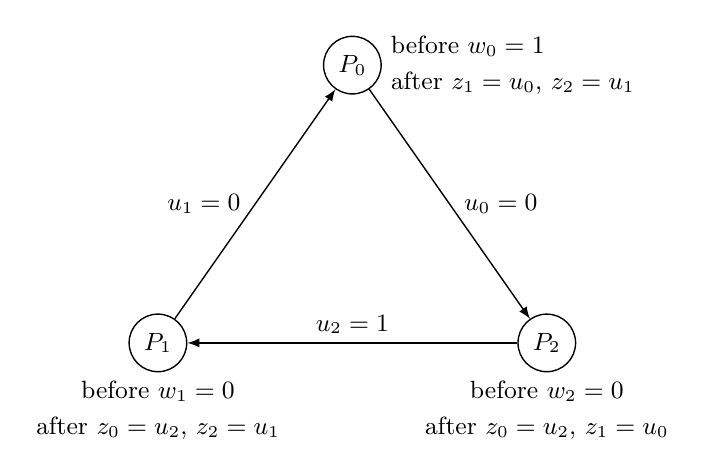
\begin{tikzpicture}[x=1bp,y=1bp,>=latex,line width=.5bp,every node/.style={font=\fontsize{9bp}{13bp}\selectfont,inner sep=3bp}]
  \node[draw,circle] (p0) at (125,100) {$P_0$};
  \node[draw,circle] (p1) at (55,0) {$P_1$};
  \node[draw,circle] (p2) at (195,0) {$P_2$};
  \draw[->] (p0) -- node[right=2bp] {$u_0 = 0$} (p2);
  \draw[->] (p1) -- node[left=2bp] {$u_1 = 0$} (p0);
  \draw[->] (p2) -- node[above] {$u_2 = 1$} (p1);
  \node[align=left,anchor=west] at (p0.east) {before $w_0 = 1$\\after $z_1 = u_0$, $z_2 = u_1$};
  \node[align=center,anchor=north] at (p1.south) {before $w_1 = 0$\\after $z_0 = u_2$, $z_2 = u_1$};
  \node[align=center,anchor=north] at (p2.south) {before $w_2 = 0$\\after $z_0 = u_2$, $z_1 = u_0$};
\end{tikzpicture}
\end{slide}

\begin{slide}[.6]{Toy MPC -- AND layers (rounds 1--4)}
\1 Layer $\ell = 1, 2, 3$
  \2 Gate $g$ computes $z^{(\ell)}_g = z^{(\ell-1)}_{2g} z^{(\ell-1)}_{2g+1} \in \mathbb F_2$
  \2 $z^{(0)}_e = b_e$
  \2 All gates of a layer reshare in one round
\1 Rerand reshares the term each $P_i$ owns
  \2 $\sh{z'}$ has fresh terms, with $z' = z^{(3)}_0$
  \2 Redundant here, but needed in the DKG for outputs\\
     linear in the PRF inputs
\1 Record 8 tuples $(x_e, y_e, z_e) \in \mathbb F_2^3$ for the check
  \2 Tuple $e = 0, \dots, 6$ holds the 2 inputs and the output of gate $e$
  \2 Tuple $e = 7$ is $(z^{(3)}_0, 1, z')$ for rerand, with $\sh{1} = (1, 0, 0)$
\side
Bits sent in rounds 1 to 4\\
\tbl{lll}{Round & Step & Each sends}{
  1 & Layer 1 & 4 bits \\
  2 & Layer 2 & 2 bits \\
  3 & Layer 3 & 1 bit \\
  4 & Rerand & 1 bit}
\tnote{Each round $P_0 \to P_2$, $P_1 \to P_0$, $P_2 \to P_1$}
\end{slide}

\begin{slide}[.6]{Toy MPC -- Check Setup (round 5)}
\1 A reshare may add errors, so check all tuples first
\1 Lift the tuples from $\mathbb F_2$ into $\mathbb F_{2^{128}}$
\1 A coin gives public random $c_0, c_1, c_2 \in \mathbb F_{2^{128}}$
  \2 $\mathsf{Rand}$ gives 2 shared elements $\gamma_0, \gamma_1$, opened as Shamir shares
  \2 Abort unless the 3 opened shares of each lie on one line
  \2 $c_k = H(\kappa, k)$ cut to 128 bits, with key $\kappa = H(\rho, \gamma_0, \gamma_1)$ of round $\rho$
  \2 Weight $\beta_e = \prod_{k : e_k = 1} c_k$ for $e = \sum_k e_k 2^k$
\1 Conv turns $\sh{v}$ into the Shamir sharing $\langle v \rangle$ locally \cite{CDI05}
  \2 $P_i$ holds $V(i+1)$ for a line $V$ over $\mathbb F_{2^{128}}$ with $V(0) = v$
  \2 $\langle A \rangle = (\beta_e x_e)_{e < 8}$, $\langle B \rangle = (y_e)_{e < 8}$ in $\mathbb F_{2^{128}}^8$
  \2 $\langle C \rangle = \bigoplus_e \beta_e z_e \in \mathbb F_{2^{128}}$
\1 Claim $C = \bigoplus_e A_e B_e$, false w.h.p.\ if any $z_e \ne x_e y_e$
\side
Messages of a coin\\
\flow{$s_0$}{$s_0$}{$s_1$}{$s_1$}{$s_2$}{$s_2$}
\tnote{$s_i$ holds the shares of $P_i$ of $\gamma_0$ and $\gamma_1$, 2 elements of $\mathbb F_{2^{128}}$\\
All operators open $\gamma_0, \gamma_1$ from $s_0, s_1, s_2$}
\vspace{16bp}Conv of each operator\\
\tbl{ll}{Operator & Shamir share $V(i+1)$}{
  $P_0$ & $v_1 \psi_1(1) \oplus v_2 \psi_2(1)$ \\
  $P_1$ & $v_0 \psi_0(2) \oplus v_2 \psi_2(2)$ \\
  $P_2$ & $v_0 \psi_0(3) \oplus v_1 \psi_1(3)$}
\tnote{$V(X) = \bigoplus_k v_k \psi_k(X)$ with $\psi_k(X) = 1 \oplus X / (k+1)$\\
So $V(0) = v$, and $\psi_k(k+1) = 0$ removes the term $P_k$ lacks}
\end{slide}

\begin{slide}[.6]{Toy MPC -- Halving (rounds 6--11)}
\1 Halve the claim $C = \bigoplus_e A_e B_e$ from 8 to 4, 2, 1 elements
\1 Split $A = (A_{\mathrm{lo}}, A_{\mathrm{hi}})$, $B$ likewise
  \2 $A'(X) = A_{\mathrm{lo}} \oplus X (A_{\mathrm{lo}} \oplus A_{\mathrm{hi}})$, $B'(X)$ likewise
  \2 $P(X) = \bigoplus_e A'(X)_e B'(X)_e$, quadratic
\1 Round 1 reshares $p_0 = P(0)$ and $p_2 = [X^2] P$ in $\mathbb F_{2^{128}}$
  \2 The claim gives $P(1) = C \oplus p_0$, so all of $P$ is shared
\1 Round 2 opens a coin $r \in \mathbb F_{2^{128}}$
  \2 Fold $A \leftarrow A'(r)$, $B \leftarrow B'(r)$
  \2 New claim $C \leftarrow P(r) = p_0 \oplus (C \oplus p_2) r \oplus p_2 r^2$
\1 A wrong claim survives with probability at most $2 / (2^{128} - 2)$
\side
Messages of a halving reshare\\
\flow{}{$u_0, u_0'$}{$u_1, u_1'$}{}{}{$u_2, u_2'$}
\tnote{$u_i, u_i'$ are the shares of $P_i$ of $p_0, p_2$, masked as in the AND gate\\
Round 2 sends a coin as in round 5}
\end{slide}

\begin{slide}[.6]{Toy MPC -- Final Check and Open (rounds 12--15)}
\1 After 3 halvings the claim is $C = ab$
\1 Round 12 takes masks $w_a, w_b \in \mathbb F_{2^{128}}$ by $\mathsf{Rand}$
  \2 Reshare $q_0 = w_a w_b$, $q_2 = (w_a \oplus a)(w_b \oplus b)$
\1 Round 13 opens a coin $r \in \mathbb F_{2^{128}}$ with digests
  \2 A digest of each held term goes to all
  \2 Abort if two holders of a term hold different copies
\1 Round 14 opens $u, v, w \in \mathbb F_{2^{128}}$, accepted iff $uv = w$
  \2 $u = w_a \oplus r (w_a \oplus a)$ and $v = w_b \oplus r (w_b \oplus b)$
  \2 $w = q_0 \oplus (C \oplus q_0 \oplus q_2) r \oplus q_2 r^2$
\1 Round 15 opens $\sh{z'}$ to get $b_0 \wedge \dots \wedge b_7 \in \mathbb F_2$
  \2 The owner sends its copy, the other holder its hash
\side
Messages of the output open\\
\flow{$H(z'_1)$}{$z'_2$}{$z'_0$}{$H(z'_2)$}{$H(z'_0)$}{$z'_1$}
\tnote{$z'_k \in \mathbb F_2$, the term that the receiver lacks\\
$H$ is a collision-resistant hash}
\end{slide}

\begin{slide}{Toy MPC -- All Messages}
\1[] Messages of each round\\
\tbl{lll}{Round & Step & Each operator sends}{
  1, 2, 3 & AND layers & 4, 2, 1 elements of $\mathbb F_2$ to next \\
  4 & Rerand & 1 element of $\mathbb F_2$ to next \\
  5, 7, 9, 11 & Coin & 2 elements of $\mathbb F_{2^{128}}$ to both others \\
  6, 8, 10 & Halving & 2 elements of $\mathbb F_{2^{128}}$ to next \\
  12 & Final masks & 2 elements of $\mathbb F_{2^{128}}$ to next \\
  13 & Coin and digests & 2 elements of $\mathbb F_{2^{128}}$ and 2 digests to both others \\
  14 & Final open & 3 elements of $\mathbb F_{2^{128}}$ to both others \\
  15 & Output open & 1 element of $\mathbb F_2$ and 1 hash}
\tnote{Next means $P_0 \to P_2$, $P_1 \to P_0$, $P_2 \to P_1$}
\end{slide}

\begin{slide}{From Toy MPC to DKG}
\1 Rounds
  \2 Grow linearly with the circuit depth
  \2 Grow logarithmically with the number of tuples in the check
\1 Batching
  \2 The check keeps every tuple until its coin opens
  \2 One check for a whole bottom tree would keep over 300 GB per operator
  \2 So each batch of 128 chains has its own check, with $1.4 \cdot 10^7$ tuples
  \2 A bottom tree has 29,696 batches, and several run at a time
\1 Reshare modes
  \2 Peer mode sends $n(t-1)$ bits per AND gate in 1 round
  \2 Collector mode sends $3(t-1)$ bits per AND gate in 2 rounds, used for $n > 3$
\1 Rounds of a batch
  \2 Depth 72 gives 72 AND rounds in peer mode and 144 in collector mode
  \2 The check takes $1 + 2 \cdot 24 + 3 = 52$ rounds for 24 halvings
  \2 Rerand and open take 1 round each, so 126 rounds for 2-of-3 and 198 for 3-of-5, 4-of-7 and 5-of-9
\end{slide}

\end{document}
